\documentclass[11pt]{article}
\usepackage{mathrsfs}
\usepackage{amssymb}
\usepackage{amsmath}
\usepackage{amsthm}
\usepackage{amscd}
\usepackage{epstopdf}
\usepackage{enumerate}
\usepackage[normalem]{ulem}
\usepackage{hyperref}
\usepackage{listings}
\usepackage{graphicx}
\usepackage{tikz}
\usepackage{amstext} % for \text macro
\usepackage{array}   % for \newcolumntype macro
\newcolumntype{L}{>{$}l<{$}} % math-mode version of "l" column type
\usepackage[normalem]{ulem}
\allowdisplaybreaks
\graphicspath{{./Images/}}
\hypersetup{
    colorlinks=true,
    linkcolor=blue,
    filecolor=magenta,      
    urlcolor=cyan,
}

\textwidth = 6.5 in
\textheight = 9 in
\oddsidemargin = 0.0 in
\evensidemargin = 0.0 in
\topmargin = 0.0 in
\headheight = 0.0 in
\headsep = 0.0 in
\parskip = 0.2in
\parindent = 0.0in
\newtheorem{theorem}{Theorem}
\newtheorem{conjecture}{Conjecture}
\newtheorem{claim}[theorem]{Claim}
\newtheorem{question}[theorem]{Question}
\newtheorem{problem}[theorem]{Problem}
\newtheorem{lemma}[theorem]{Lemma}
\newtheorem{proposition}[theorem]{Proposition}
\newtheorem{observation}[theorem]{Observation}
\newtheorem{corollary}[theorem]{Corollary}
\newtheorem{Theorem}{Theorem}[section]
\newtheorem{Claim}[Theorem]{Claim}
\newtheorem{Lemma}[Theorem]{Lemma}
\newtheorem{Proposition}[Theorem]{Proposition}
\newtheorem{Corollary}[Theorem]{Corollary}
\newtheorem{definition}[theorem]{Definition}
\newtheorem{example}{Example}
\newtheorem{assumption}{Assumption}
\newtheorem{aside}{Aside}
\newtheorem{fact}{Fact}


\theoremstyle{definition}
\newtheorem{exercise}[theorem]{Exercise}
\newtheorem{remark}[theorem]{Remark}
\newcommand{\N}{\mathbb{N}}
\newcommand{\Q}{\mathbb{Q}}
\newcommand{\Z}{\mathbb{Z}}
\newcommand{\R}{\mathbb{R}}
\newcommand{\C}{\mathbb{C}}
\newcommand{\F}{\mathbb{F}}
\newcommand{\Hom}{\mathrm{Hom}}

\title{FiveThirtyEight's Febuary 11, 2022 Riddler}
\author{Emma Knight}
\date{\today}
\begin{document}
\maketitle
This week's riddler, courtesy of Dean Ballard, is about primes and cubes:
\begin{question}
Consider a cube, which has eight vertices, or corners. Suppose I assign a prime number to each vertex. A ``face sum'' is the value I get when I add up all four prime numbers on one of the six faces.

Can you find eight primes and arrange them on a cube so that the six face sums are all equal?

\emph{Extra credit}: Can you find another set of eight primes that can similarly be arranged on the vertices of a cube? How many more can you find?
\end{question}

I will explain how to generate a lot of these cubes, and then give some examples.  Choose prime numbers $p_1, p_2, p_3$, and $p_4$, as well as an integer $n$, such that $p_i + n$ is also prime for all $i$, and the eight primes generated this way are distinct.  Then, one creates the following cube:

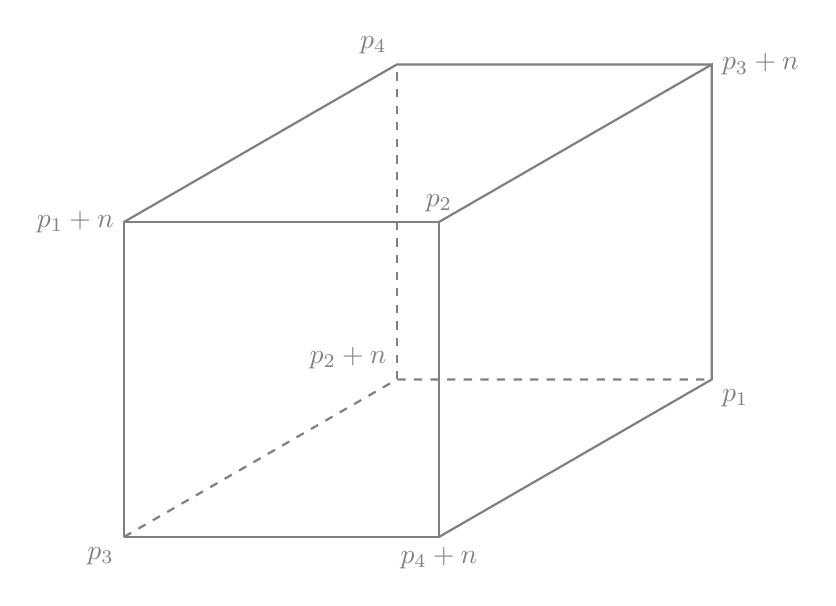
\begin{tikzpicture}
\draw[gray, thick] (0, 0) node[anchor=north east] {$p_3$} -- (0, 4) node[anchor=east] {$p_1+n$} -- (4, 4) node[anchor=south] {$p_2$} -- (4, 0) node[anchor=north] {$p_4+n$} -- (0,0);
\draw[gray, thick] (4, 0) -- ({4+sqrt(12)}, {2}) node[anchor=north west] {$p_1$} -- ({4+sqrt(12)}, {6}) node[anchor=west] {$p_3+n$} -- (4, 4);
\draw[gray, thick] (0, 4) -- ({sqrt(12)}, {6}) node[anchor=south east] {$p_4$} -- ({4+sqrt(12)}, {6});
\draw[gray, thick, dashed] (0, 0) -- ({sqrt(12)}, {2}) node[anchor=south east] {$p_2 + n$} -- ({sqrt(12)+4}, {2});
\draw[gray, thick, dashed] ({sqrt(12)}, {2}) -- ({sqrt(12)}, {6});
\end{tikzpicture}

On this cube, every face sums to $p_1 + p_2 + p_3 + p_4 + 2n$.  To get an example of this, take $p_1 = 3$, $p_2 = 11$, $p_3 = 17$, $p_4 = 29$, and $n = 2$.  There are a \emph{lot} of examples, and you are invited to do a brute force search to find as many as you please.  To give context for just how many such cubes there are, looking through the first $15$ odd primes (i.e. the primes up to $53$), there are $173$ such cubes (this counts two layouts that are symmetrical but aren't literally the same primes on the same verticies as the same cube).  Adding the next prime into the list ups this number to $286$\footnote{Adding in $61$ as well gives $376$ total cubes}, so it is not hard to find as many as you want using straight up brute force.

To see why this every such cube is of this form, notice that setting two adjacent faces to sum to the same number is the same thing as setting two opposite parellel sides to sum to the same number, and this is the same thing as setting two diagonal differences to be the same (suitably oriented).  This gives that every diagonal difference is the same (again suitably oriented), and shows that every solution is of this form.

Finally, here is my python brute force code:
\begin{verbatim}
import itertools

primes = [3, 5, 7, 11, 13, 17, 19, 23, 29, 31, 37, 41, 43, 47, 53, 59, 61]

octuples = itertools.permutations(primes, 8)
valid = []

for l in octuples:
    if ((l[0] + l[1] == l[4] + l[5]) and
        (l[2] + l[3] == l[6] + l[7]) and
        (l[0] + l[3] == l[5] + l[6]) and
        (l[1] + l[2] == l[4] + l[7])):
        valid.append(l)
        print(l)

print(len(valid)//48)
\end{verbatim}
\end{document}